\documentclass[tikz]{standalone}
\usepackage{tikz}
\usetikzlibrary{patterns,snakes}
 
\begin{document}
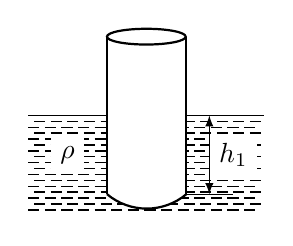
\begin{tikzpicture}
	\draw (0,0) -- (1,0);
	\draw (2,0) -- (3,0);
	\draw [thick] (1.5,1) ellipse (0.5 and 0.1);
	\draw [thick] (1,-1) arc (230:310:0.785);
	\draw [thick] (1, -1) -- (1,1);
	\draw [thick] (2, -1) -- (2,1);
	\draw (2,-1) -- (2.6,-1);
	\clip (1,-1) arc (230:310:0.785) -- (2,0) -- (3,0) -- (3,-1.3) -- (0,-1.3) -- (0,0) -- (1,0) -- cycle;
	\foreach \n [count=\k from 0] in {0,1,...,7}
    {
	    \draw[line width = 0.5pt,dash pattern = on 4pt off 2pt](0,-1.2+0.15*\k ) -- ++ (2.9,0);
	    \draw[line width = 0.5pt,dash pattern = on 4pt off 2pt](0.075,-1.2+ 0.075+0.15*\k ) -- ++ (2.9,0);
	}
	\node at (0.5, -0.5) [fill = white] {$\rho$};
	\draw [arrows={latex-latex}] (2.3, -1) -- (2.3, 0) node [midway, right, fill=white]  {$h_1$};
\end{tikzpicture}
\end{document}